\documentclass[a4paper,twoside,10pt]{report}
\usepackage{geometry}
\usepackage[utf8x]{inputenc}
\usepackage[ngerman]{babel}
\usepackage[german,figure,linesnumbered,lined]{algorithm2e}
\usepackage{tikz}
\usepackage{tkz-fct}
\usepackage{color}
\usepackage{graphics}
\usepackage{graphicx}
\usepackage{amssymb}
\usepackage{amsmath}
\usepackage{listings}
\usepackage{booktabs}
\usepackage{pdfpages}
\usepackage{pgfplots}
\usepackage{float}
\geometry{top=25mm, left=25mm, right=25mm, bottom=30mm}
\lstset{language=C++}
\setlength{\columnsep}{3em}

\begin{document}

\begin{titlepage}
\center
\Large DSEA WS 12-13\large \\[2em]
Dozent:\\Elmar Schömer\\[2em]
Mitschrift von:\\André Groß\\[2em]
Zuletzt Aktualisiert:\\\today\\

\includegraphics[scale=.2]{figures/uni_logo.png}\\[3em]
\Large \textbf{Zusammenfassung:}\\[1em]
\parbox{0.75\textwidth}{\large
Im Mittelpunkt der Veranstaltung stehen Methoden zur Entwicklung (vor allem \mbox{zeit-)} effizienter Algorithmen. Dabei betrachten wir insbesondere solche Datenstrukturen, die eine effiziente Verwaltung von dynamischen Datenmengen ermöglichen. Ein Teil der Algorithmen und Datenstrukturen wird in den Übungen implementiert.\\[.5em]

Mit dem Studium dynamischer Datentypen sowie weiterer Algorithmen schließt die Veranstaltung direkt an Einführung in die Programmierung bzw. Einführung in die Softwareentwicklung an. Allerdings werden nun mathematische Methoden zur Analyse von Algorithmen (Korrektheit und vor allem Aufwand) eingesetzt.\\[.5em]

http://cg.informatik.uni-mainzde/dsea\\
\textbf{Raum:} Mi C02, Mo 03-428\\
\textbf{Abgabe:} Mittwochs 12:00\\
\textbf{Sprache:} Grundsätzlich Java, ggf auch Python
}
\end{titlepage}
\normalsize
\tableofcontents
\twocolumn

\part{Skriptum}
\include{skriptum}
%%%%%%%%%%%%%%%%%%%%%%%%%%%%%%%%%%%%%%%%%%%%%%%%%%%%%%%
\part{Die letzte(n) Vorlesung(en)}
\section{AVL \, Bäume \, Wiederholung}

Die Logaritmische Tiefe ist wichtig für die Suchzeit usw.\\
Linker und Rechter Teilbaum dürfen sich für Suche usw. in ihrer Tiefe nur um max. Eins unterscheiden.

\chapter{VL 19.11.2012}
\begin{align*}
f(z) &=(z+c)^p \\
&=\sum_{n=0}^\infty \frac{1}{n!}f^{(n)}(z0)(z-z_0)\\
\mbox{wähle }&z0=0\\
f'(z)&=p(z+c)^{p-1}\\
f''(z)&=p(p-1)(z+c)^{p-2}\\
f^{(n)}(z)&=p(p-1)(p-2)\hdots(p-n+1)(z+c)^{p-n}\mbox{(Taylor)}\\
\mbox{hier fehlt was!}
\end{align*}

\begin{align*}
b_0=1,b_n&=\sum_{i=1}^nb_{i-1}b_{n-i}\\
B(z)&=\sum_{n=0}^\infty b_nz^n\Rightarrow B(z)\frac{1-\sqrt{1-4z}}{2z}\\
\sqrt{1-4z}&=(1-4z)^\frac{1}{2}\\
&=\sum_{n=0}^\infty \left(\begin{array}{c}\frac{1}{2}\\n\end{array}\right)1^{\frac{1}{2}-n}(-4z)^n\\
&=\sum_{n=0}^\infty\begin{array}{c}\frac{1}{2}\\n\end{array}(-4)^nz^n\\
&=1+\sum_{n=0}^\infty \begin{array}{c}\frac{1}{2}\\n\end{array}(-4)^nz^n\\
&=1+\sum_{n=0}^\infty \begin{array}{c}\frac{1}{2}\\n+1\end{array}(-4)^{n+1}z^{n+1}
\end{align*}

hier fehlt auch noch ne Menge...
\[b_n=-\frac{1}{2}\begin{array}{c} \frac{1}{2} \\n+1\end{array}(-4)^{n+1}\]
den rest kann ich nicht lesen....

\section{Bijektion \, zwischen \, Binärbäumen}
\[n=3; c_c=\frac{1}{n+1}\begin{array}{c} 2n\\n\end{array}\Rightarrow c_3=5\]
Graphik

\section{Amortisierte Analyse am Beispiel von 2-5-Bäumen}
a-b-Bäume: Jeder Knoten Des Baumes hat mind a Kinder und Höchstens b Kinder.
Blattorientierte Speicherung der zu verwaltenden Elemente
\begin{figure}[H]
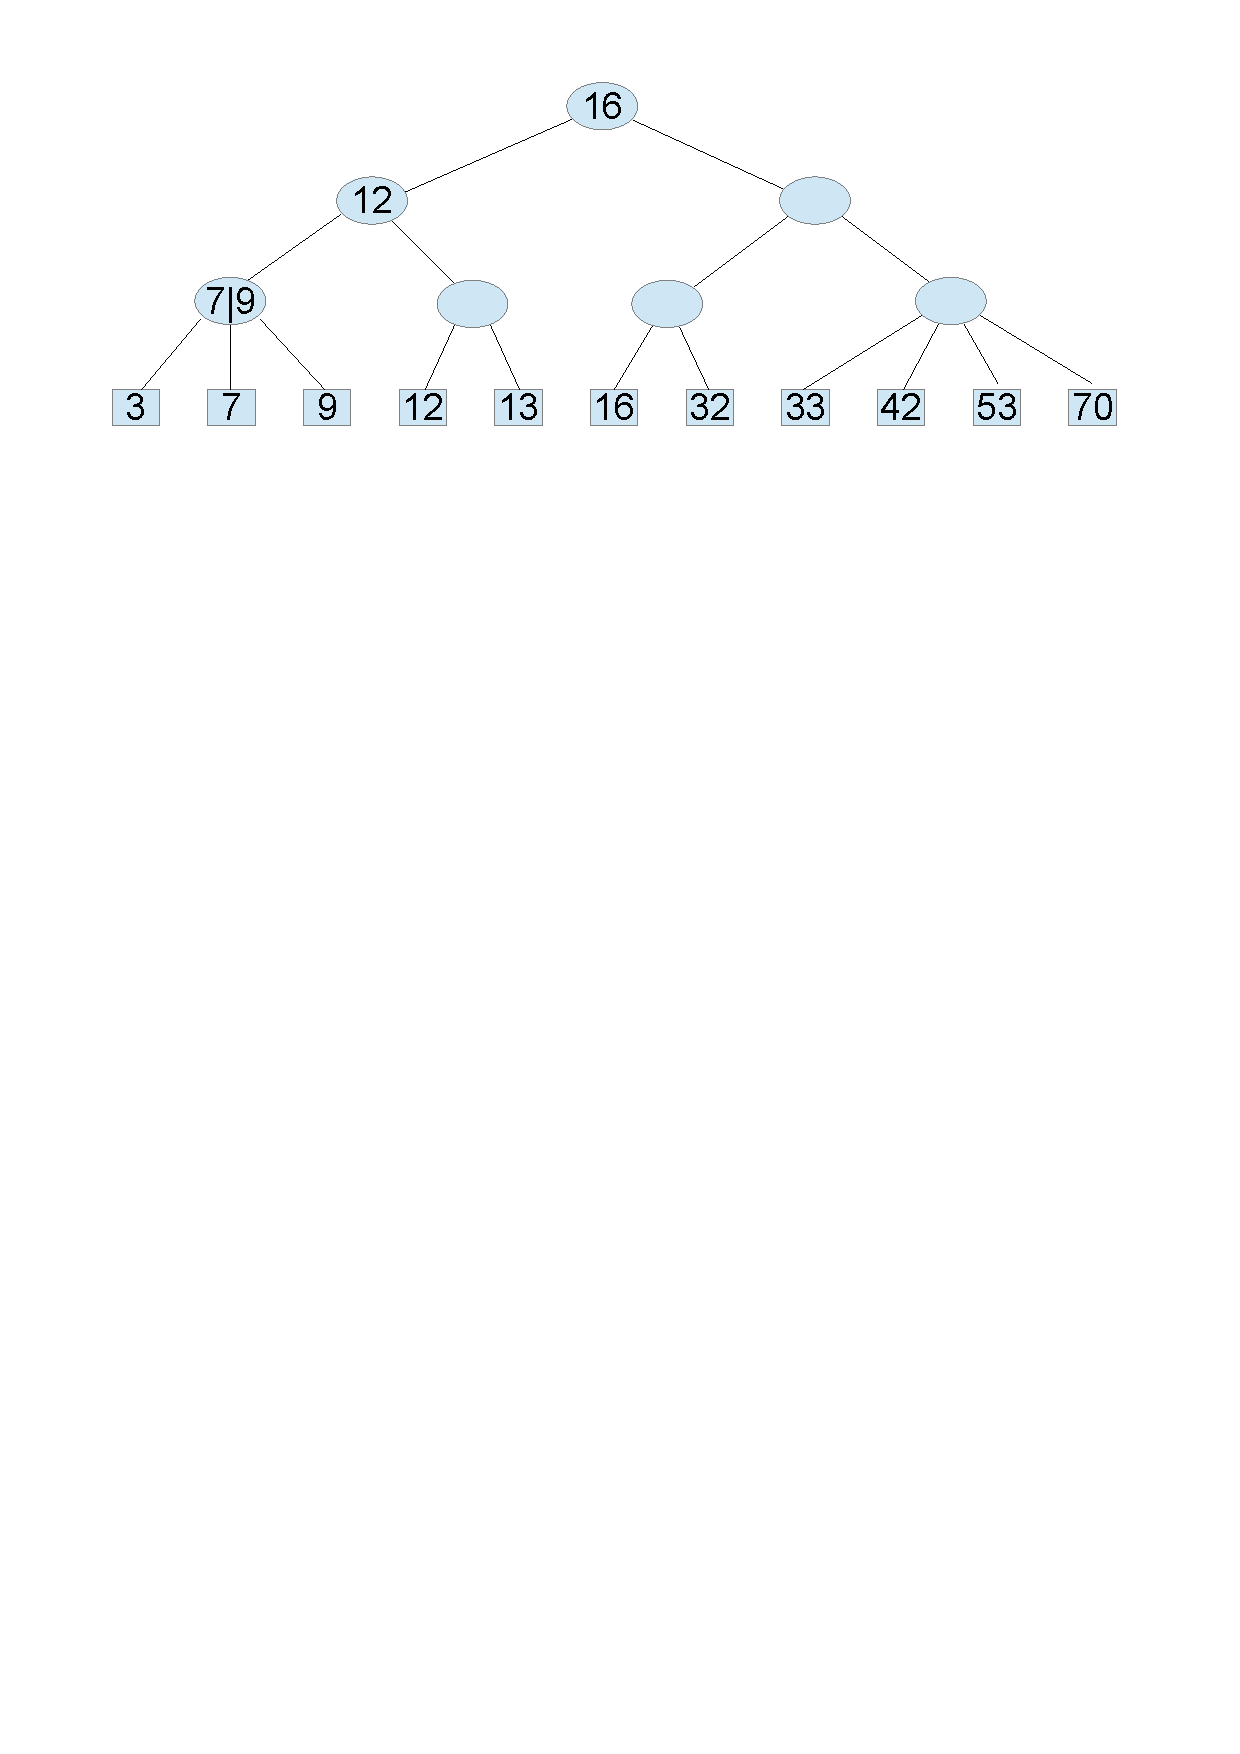
\includegraphics[trim= 1.8cm 20cm 2cm 1.3cm,clip,width=\columnwidth]{figures/aa25baum.pdf}
\caption{2-5-Baum}
\end{figure}
Zahl der Blätter n :
\[2^t\le n\le 5^t\]
\[\log_5n \le t\le  \log_2n\]
\[\Rightarrow t\in \theta (\log n)\]

Strategie zum Einfügen und Löschen von Elementen

\begin{figure}[H]
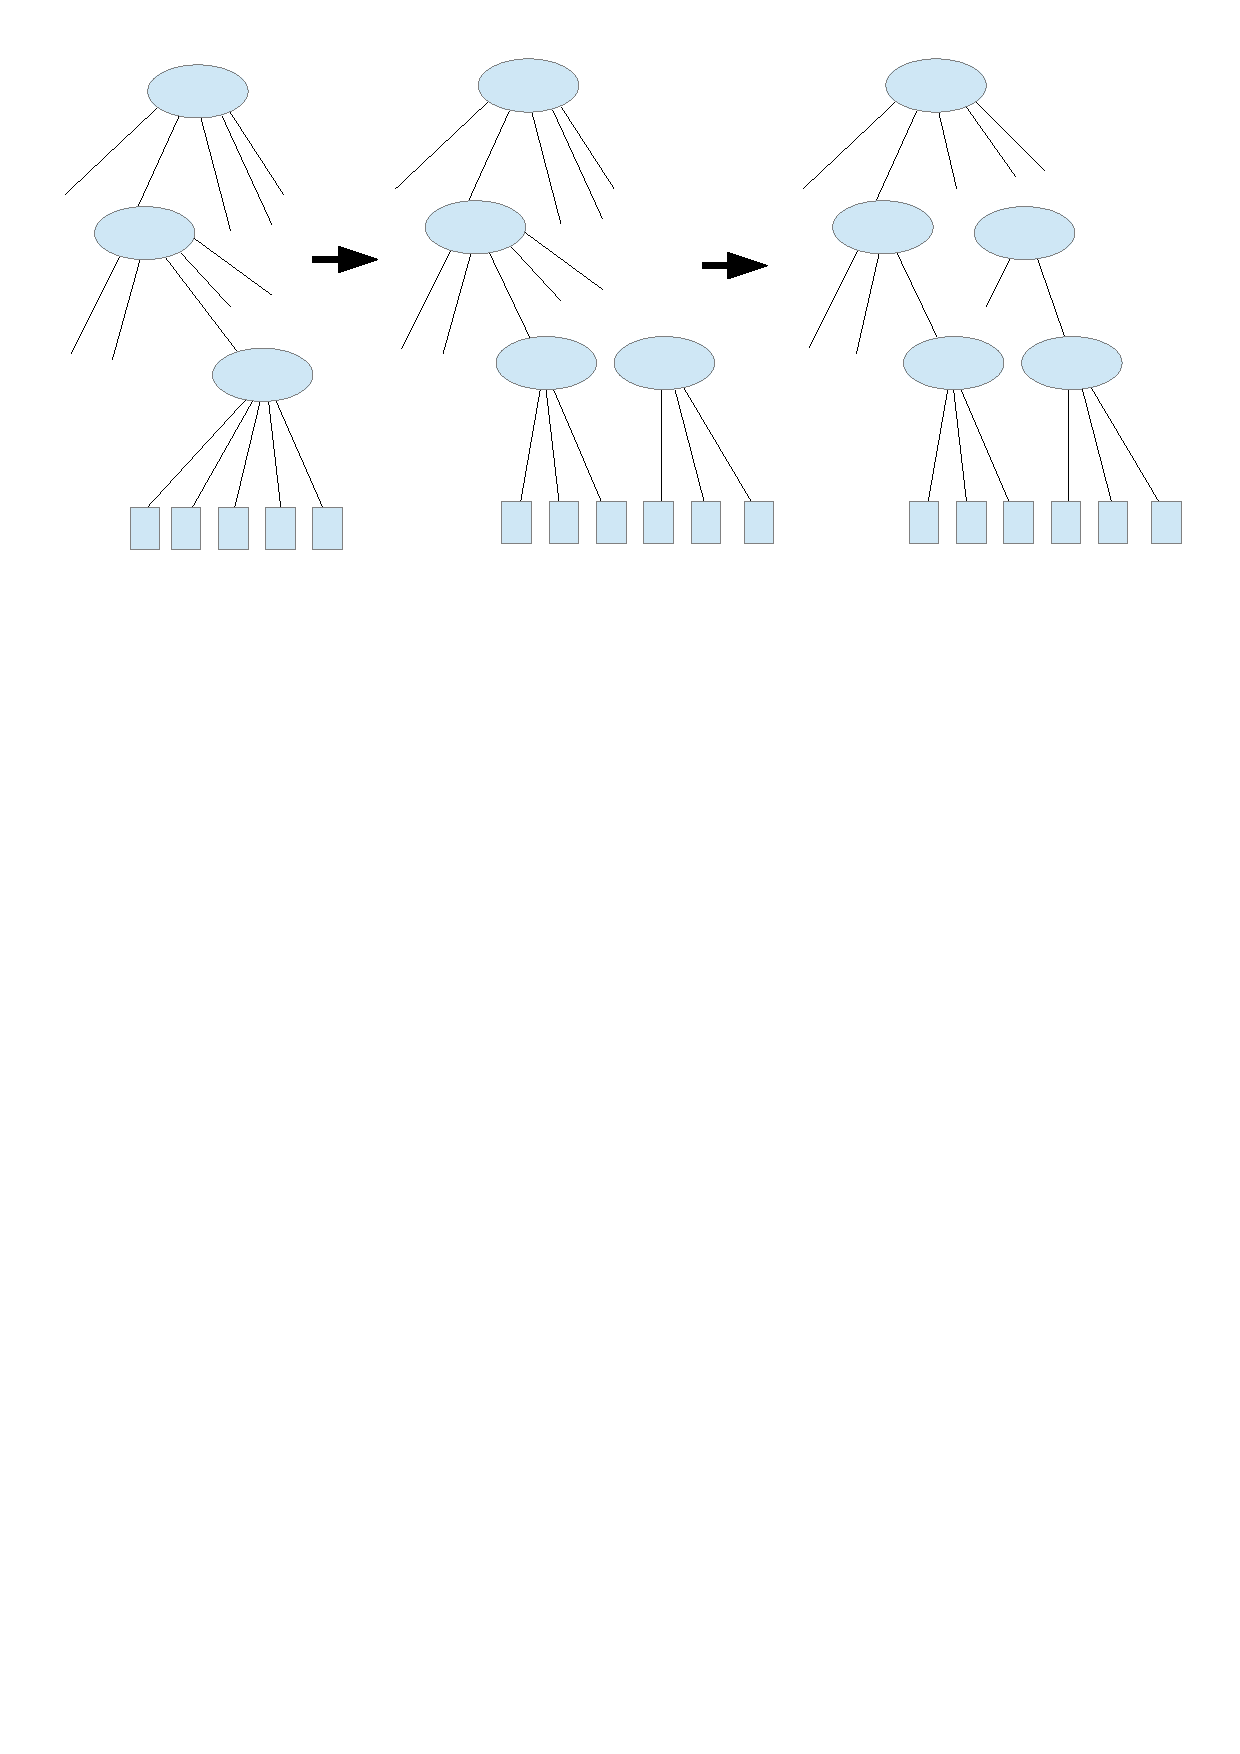
\includegraphics[trim= 1cm 20cm 1cm 1cm,clip,width=\columnwidth]{figures/25bauminsert.pdf}
\caption{Einfügen in 2-5-Baum}
\end{figure}

Beim Löschen von Elementen kann eine Kaskade Von Fusionsoperatoren auf dem Suchpfad notwendig werden. Ggf. Wurzel löschen und Kinder Zusammenlegen.

Laufzeit für Suchen, Einfügen, Löschen $\in \theta(\log n)$

\chapter{VL 21.11}
\section{Amortisierte Analyse am Beispiel des Binärzählers}

\begin{figure}[H]\center
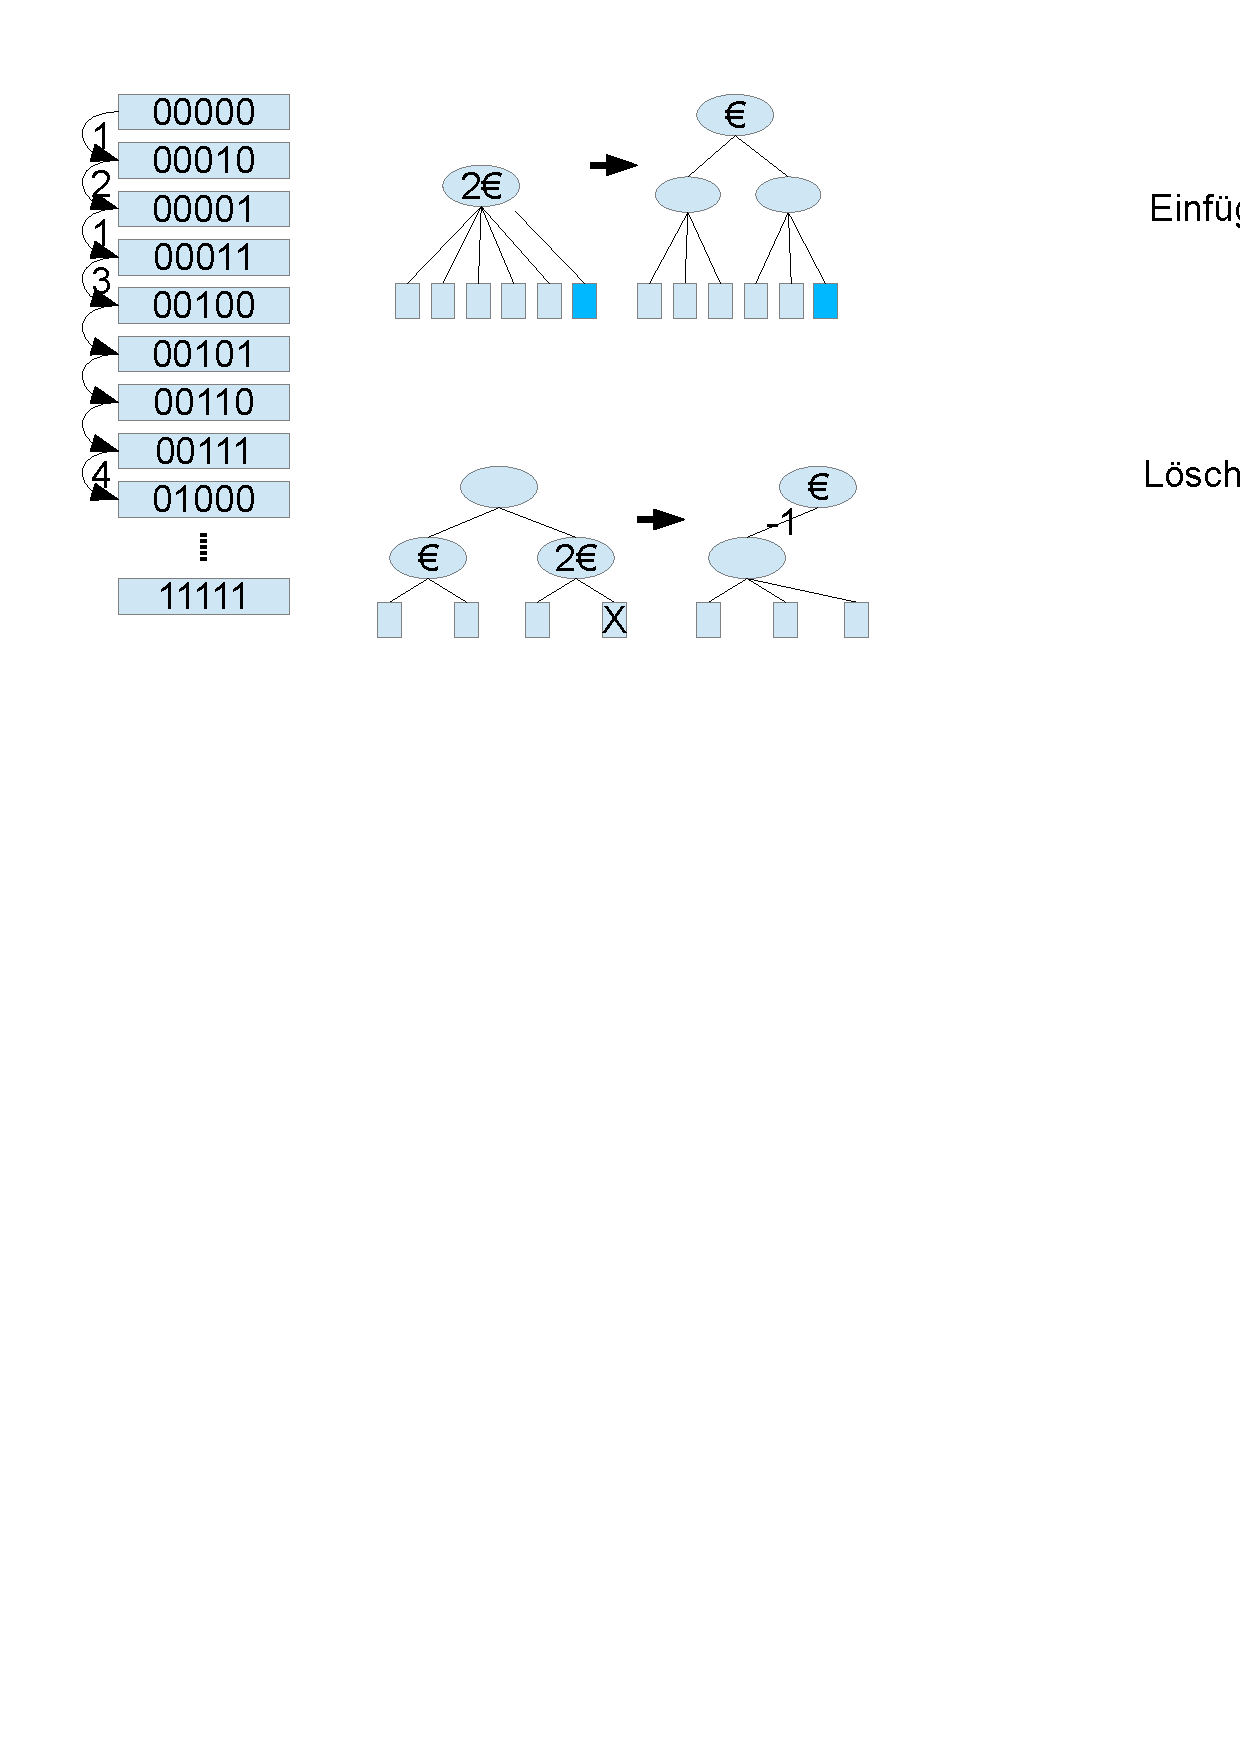
\includegraphics[trim= 1cm 18cm 15cm 1cm,clip,width=0.5\columnwidth]{figures/zaehler.pdf}
\caption{Binärzähler}
\end{figure}

Worst case Kosten einer Inkrement- Operation $$\mathcal O(\log_2n)$$\\
Gesamtkosten für eine Folge von n Inkrement- Operationen (beginnend beim Zählerstand 0)
\begin{align*}
&\frac{n}{2}&\mbox{verursachen Kosten }&1&\mbox{Endung }&0\\
&\frac{n}{4}&\mbox{verursachen Kosten }&2&\mbox{Endung }&01\\
&\frac{n}{8}&\mbox{verursachen Kosten }&3&\mbox{Endung }&011\\
&\frac{n}{16}&\mbox{verursachen Kosten }&4&\mbox{Endung }&0111\\
\end{align*}

Gesamtkosten:\\
\[\le \sum_{i=1}^\infty i\frac{n}{2^i}=n\sum_{i=1}^\infty i\left(\frac{1}{2}\right)^i =2n\]

\fbox{\parbox{\columnwidth}{ Nebenrechnung:\small
\begin{align*}
x\sum_{i=1}^\infty ix^{i-1}&=x\left(\sum_{i=0}^\infty x^i\right)'\\
&=x\left(\frac{1}{1-x}\right)'\\
&=\frac{x}{(1-x)^2}
\end{align*}
}}

\subsection{Kontomethode}
\begin{align*}
Konto(i)&= \mbox{Kontostand vor der i-ten Operation}\\
cost(i)&=\mbox{tatsächliche Kosten der i-ten Operation}\\
\sum_{i=1}^n cost(i)&=\sum_{i=1}^n Konto(i)-Konto(i+1)+a(i)\\
a(i)&=\mbox{ammotisierte Kostender i-ten Operation}\\
\Rightarrow \sum_{i=1}^n cost(i)&=Konto(i)-Konto(n+1)+\sum_{i=1}^n a(i)
\end{align*}

\subsection{amortisierte Analyse der Rekonstruierungskosten für eine Folge von m Einfüge- oder Löschoperationen in einem 2-5-Baum}
Ausgangspunkt: leerer Baum\\
Nicht betrachtet werden die Suchkosten. Wir konzentrieren uns auf die Split- und Fusions-Operationen.\\[.5em]
Kontoführung:\\
\begin{tabular}{rcccccc}
Knotengrad&1&2&3&4&5&6\\
Sparbetrag&2&1&0&0&1&2
\end{tabular}\\[.5em]
Sparplan:\\
$2RE$ pro Einfüge- bzw.Löschoperation\\
$a_i=2$\\
\textbf{Einfügen:}
\begin{figure}[H]\center
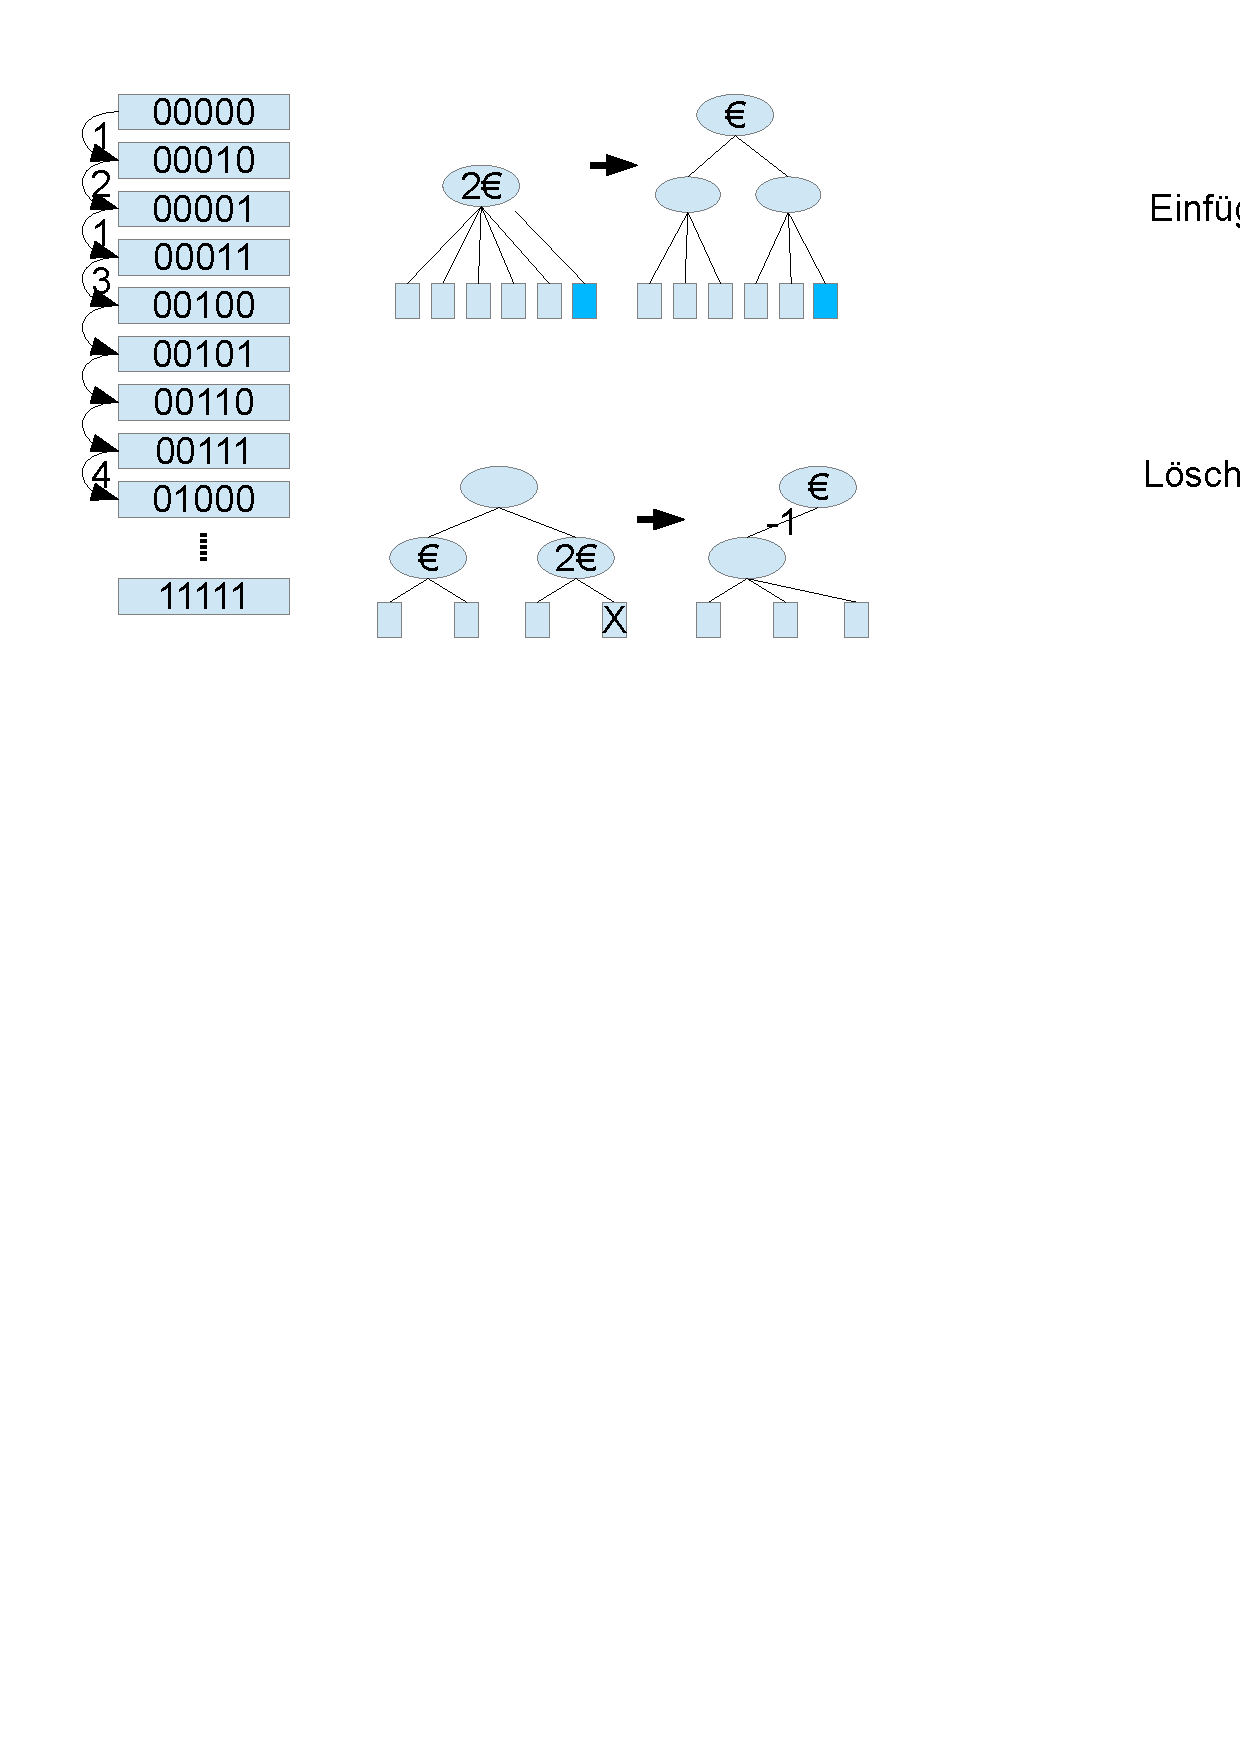
\includegraphics[trim= 6cm 24cm 6cm 1cm,clip,width=\columnwidth]{figures/zaehler.pdf}
\caption{Kosten 2-5-Baum einfügen}
\end{figure}
\textbf{Löschen:}
\begin{figure}[H]\center
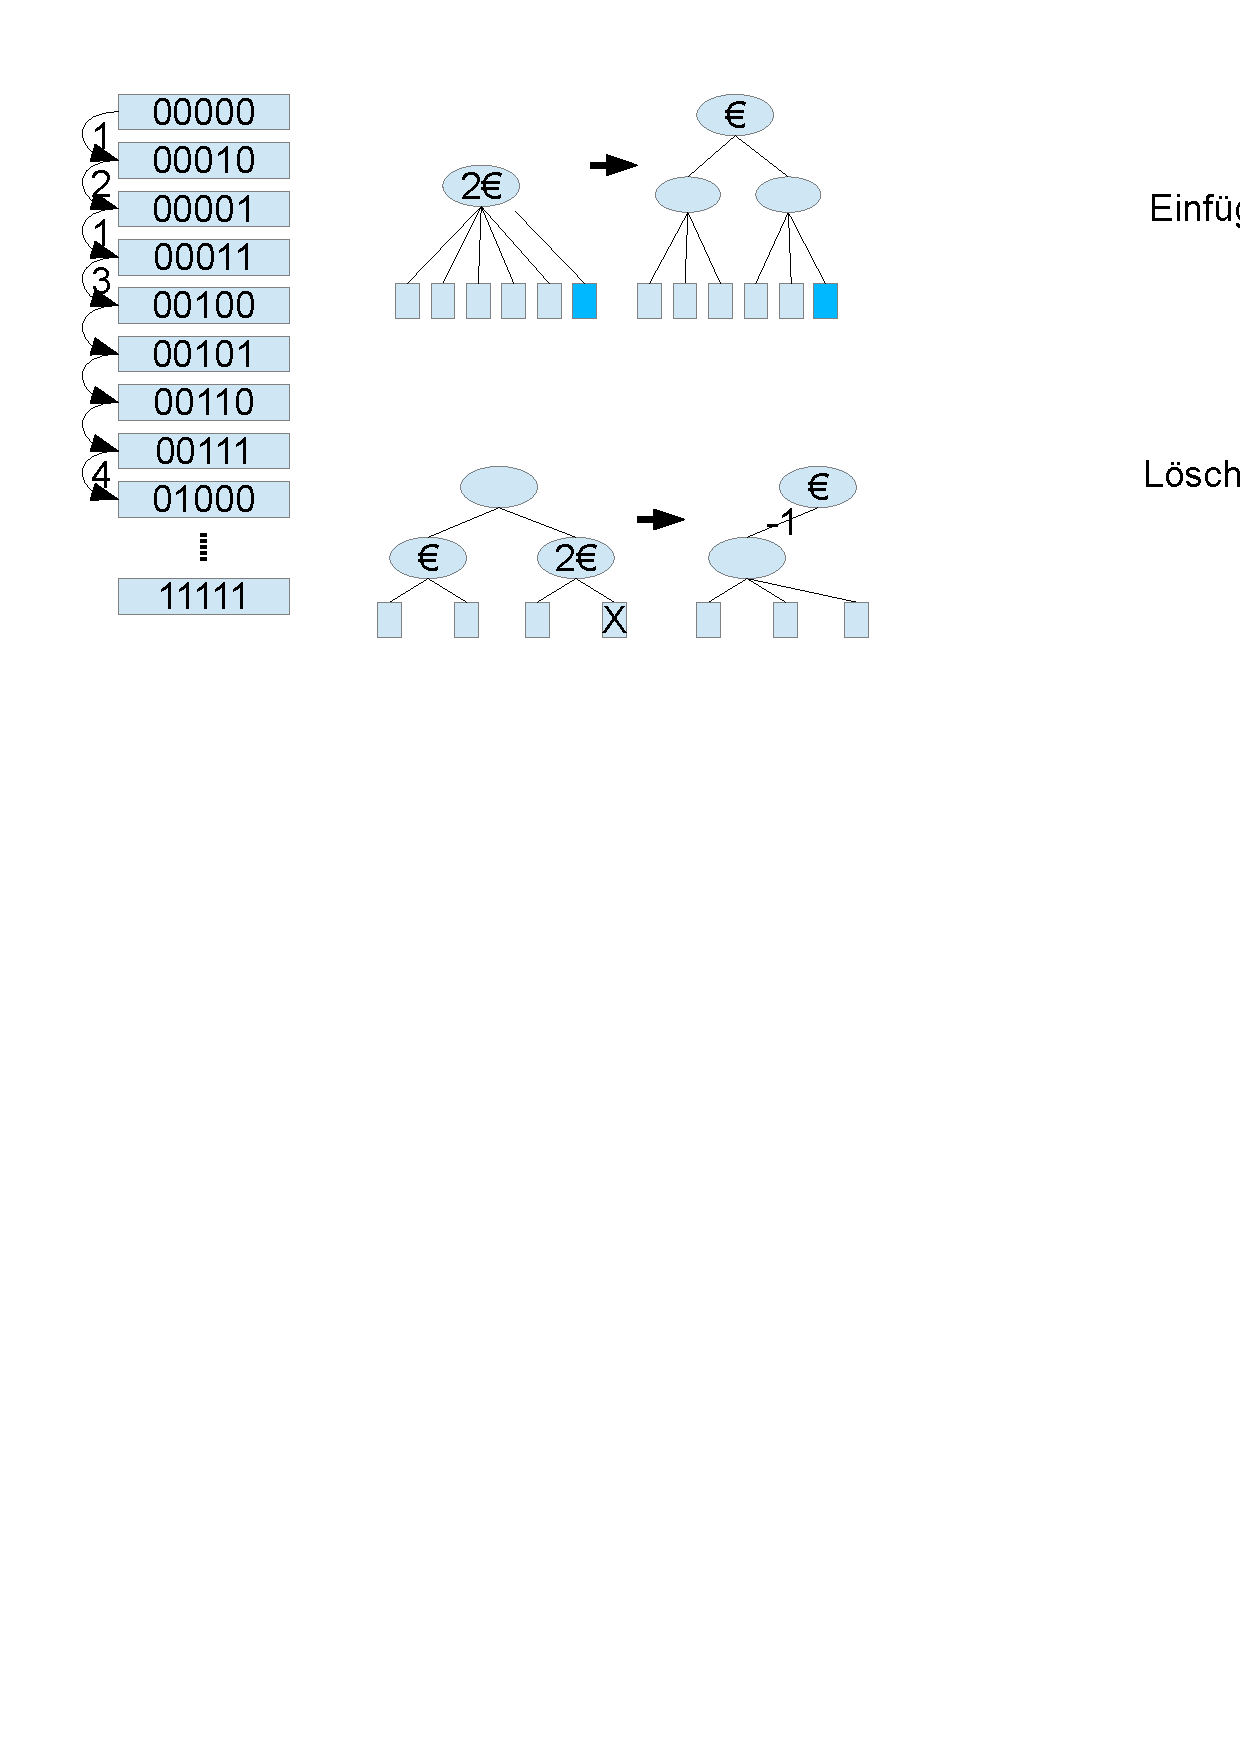
\includegraphics[trim=  6cm 18.5cm 6cm 7cm,clip,width=\columnwidth]{figures/zaehler.pdf}
\caption{Kosten 2-5-Baum Löschen}
\end{figure}

Die m Einfüge- und Löschoperationen auf einem anfangs leeren Baum haben amotisierte Kosten=2.
$\Rightarrow$ Rekonstruierungskosten insgesamt belaufen sich auf $2m$

\section{VL 26.11.}
\subsection{Skiplisten}
\begin{figure}[H]
\begin{verbatim}
class ListNode{
   int kex;
   ListNode next,down;

   boolean search(int x){
      ListNode node = head;
      do{
          while(x>node.next.key)
            node=node.next;
         if (x == node.next.key)
            return true;
         node = node.down; 
      }while(node!=null)
      return false;
      }
}
\end{verbatim}
\caption{Skiplisten Pseudocode}
\end{figure}

\begin{figure}[H]\center
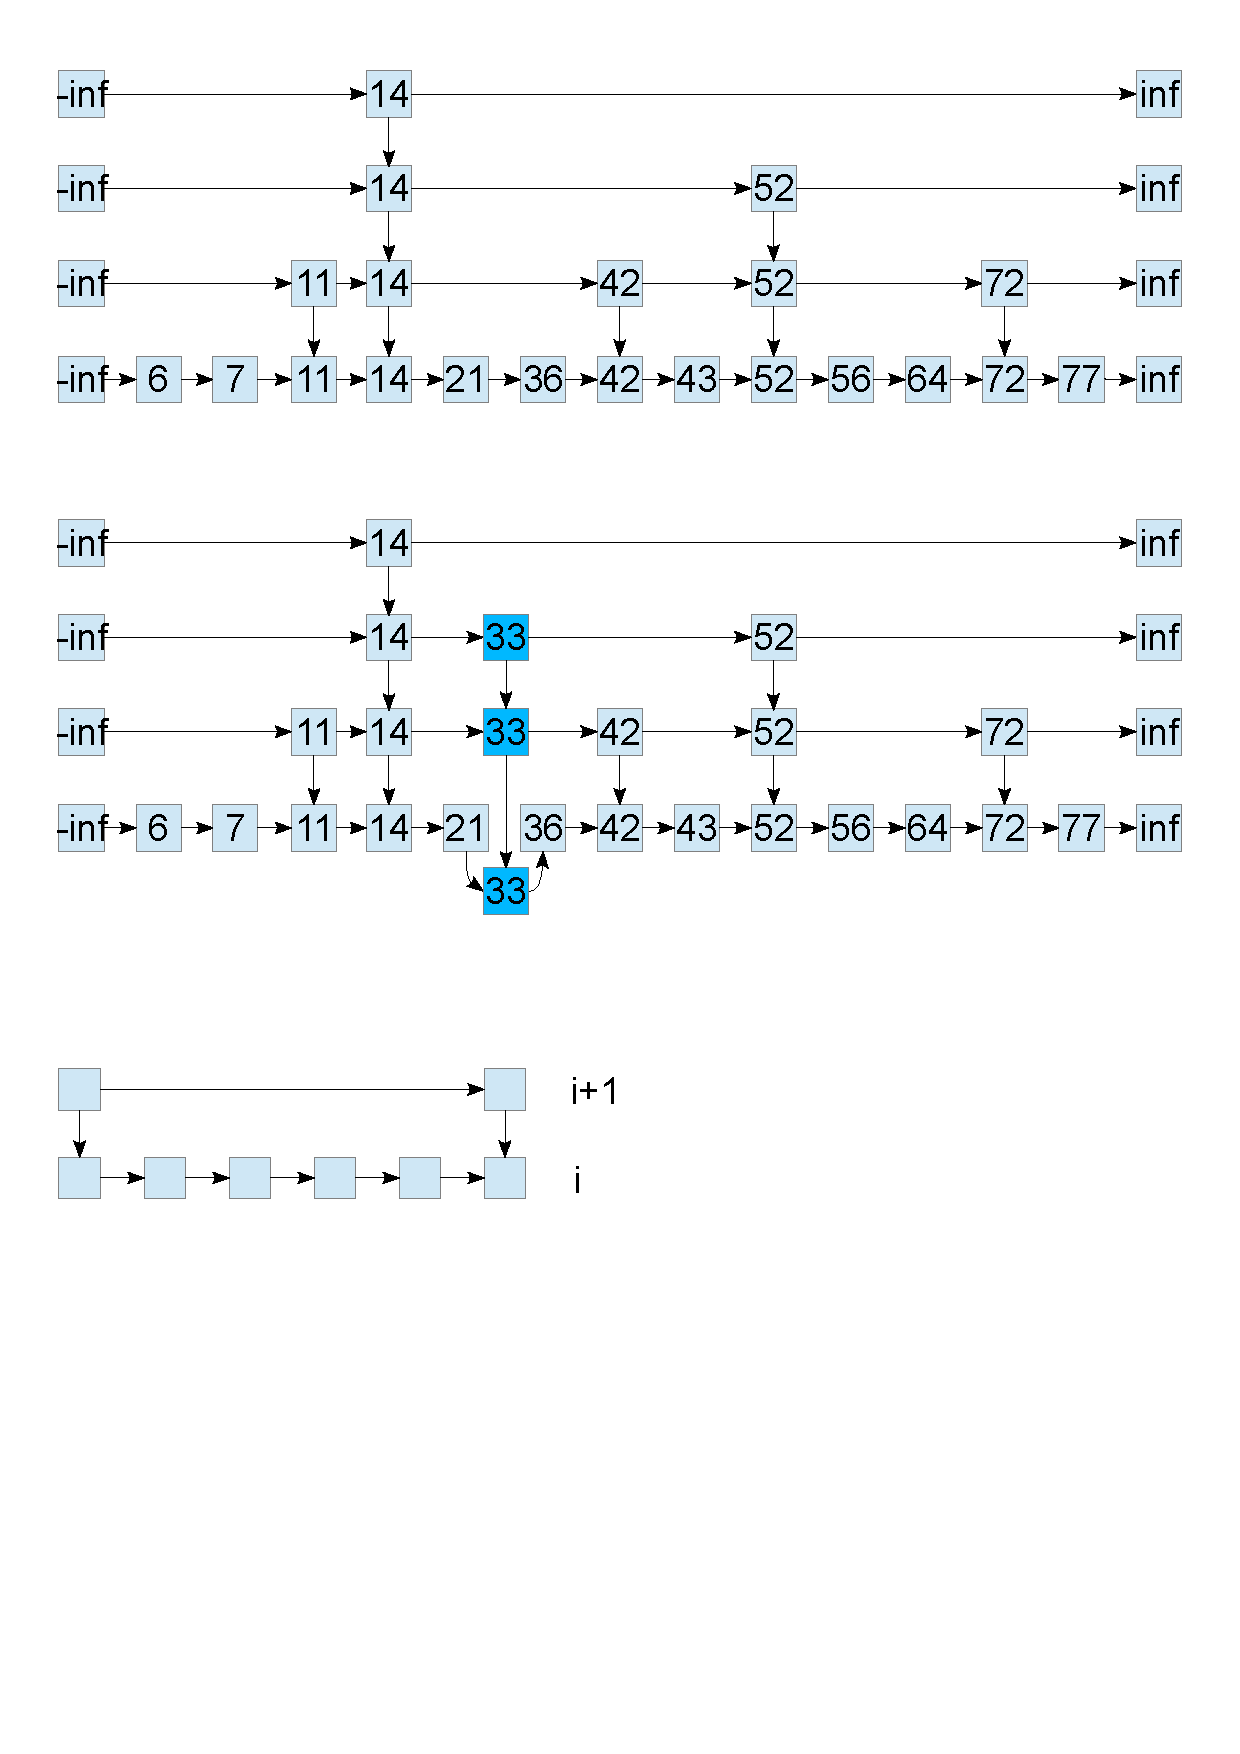
\includegraphics[trim= .9cm 22cm .9cm 1cm,clip,width=\columnwidth]{figures/skiplist.pdf}
\caption{Skipliste, ein Beispiel}
\end{figure}

\begin{figure}[H]\center
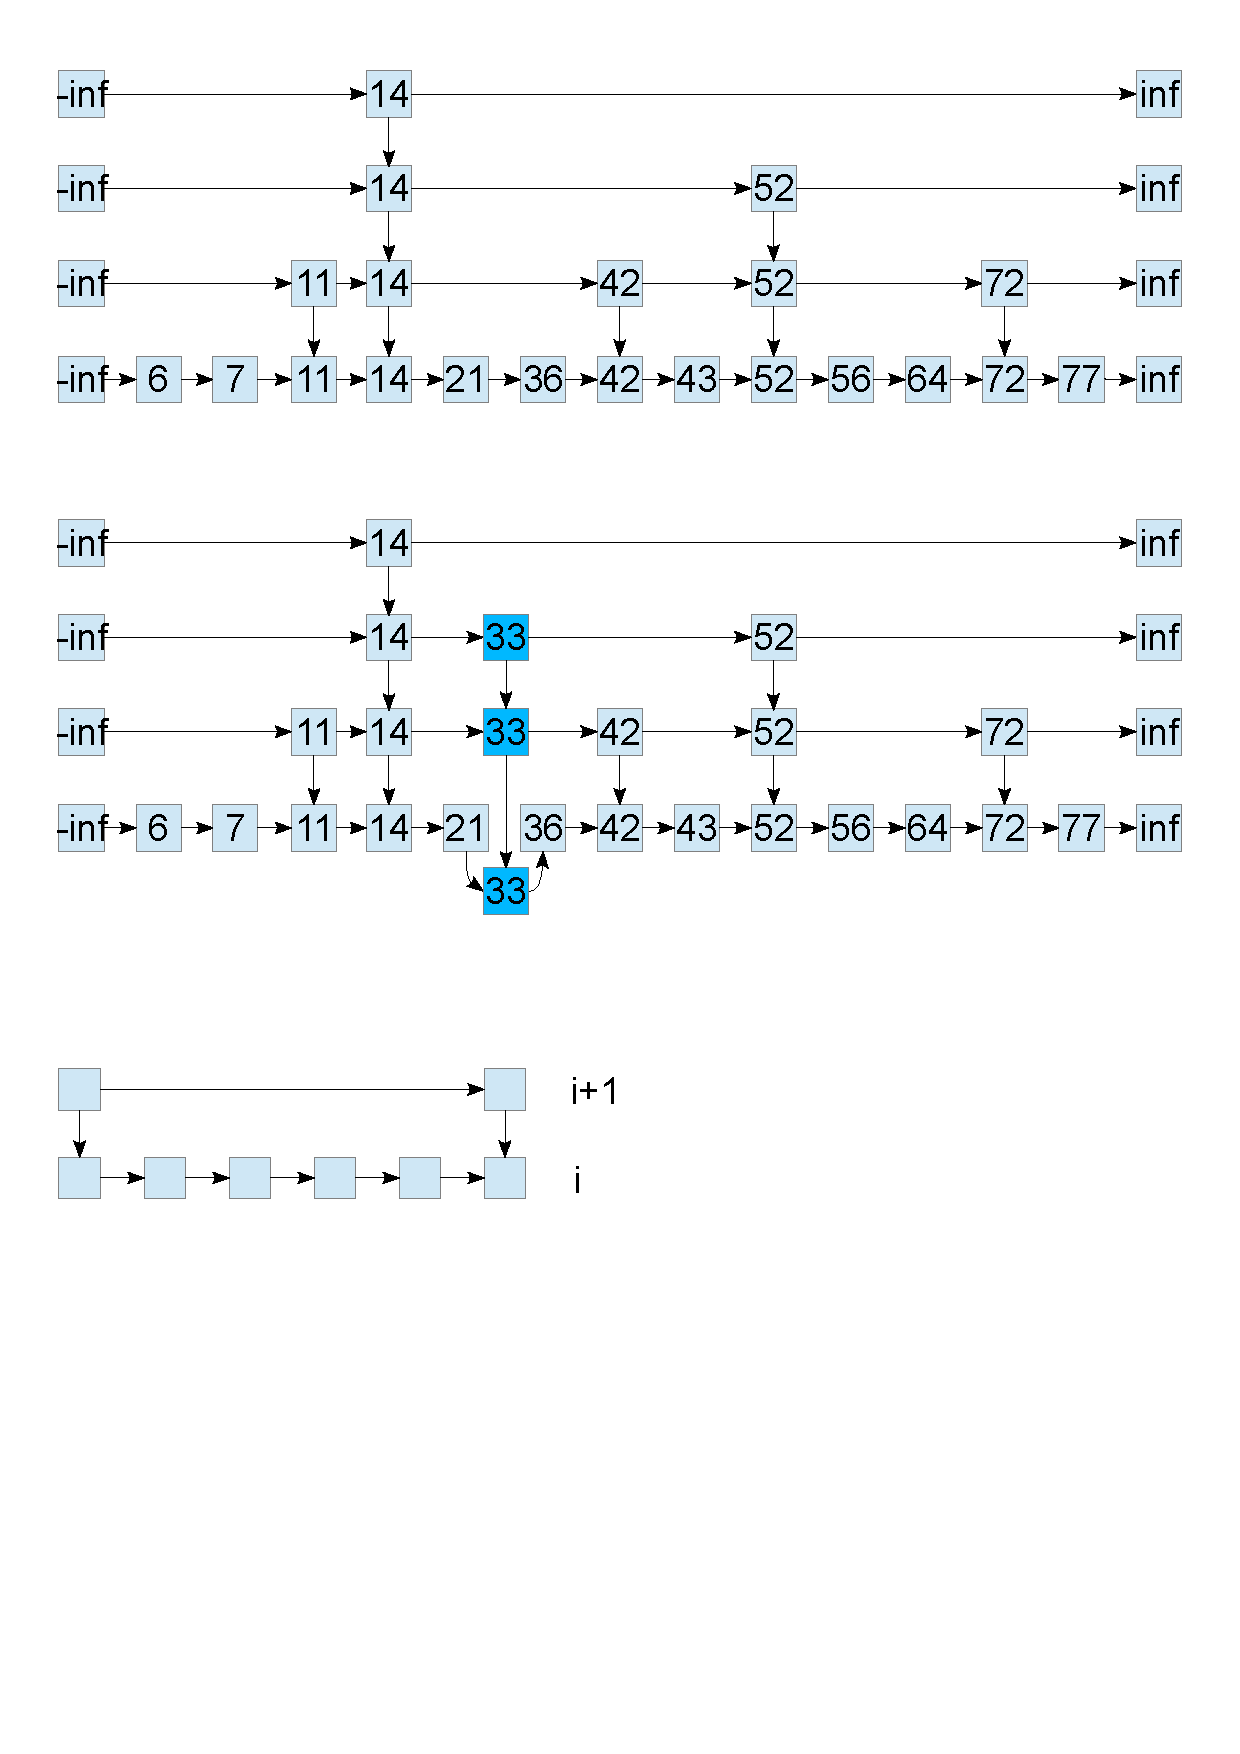
\includegraphics[trim= .9cm 14cm .9cm 8cm,clip,width=\columnwidth]{figures/skiplist.pdf}
\caption{In Skipliste einfügen}
\end{figure}

Erwartete Tiefe:\\
mit Wahrscheinlichkeit $p$ soll ein Element von Level $i$ auf Level $i+1$ angehoben werden\\
Erwartete Zahl von Elementen auf Level $i$: \, $p^in$
\[p^in<1 \Rightarrow n < \left(\frac{1}{p}\right)^i \Rightarrow i>\log_\frac{1}{p}n\]

Suchzeit:\\
Wir müssen die Ebenen von oben nach unten durchlaufen.\\
Die Frage ist, wie viele Elemente bei der verfeinerten Liste hinzukommen.\\
\begin{figure}[H]\center
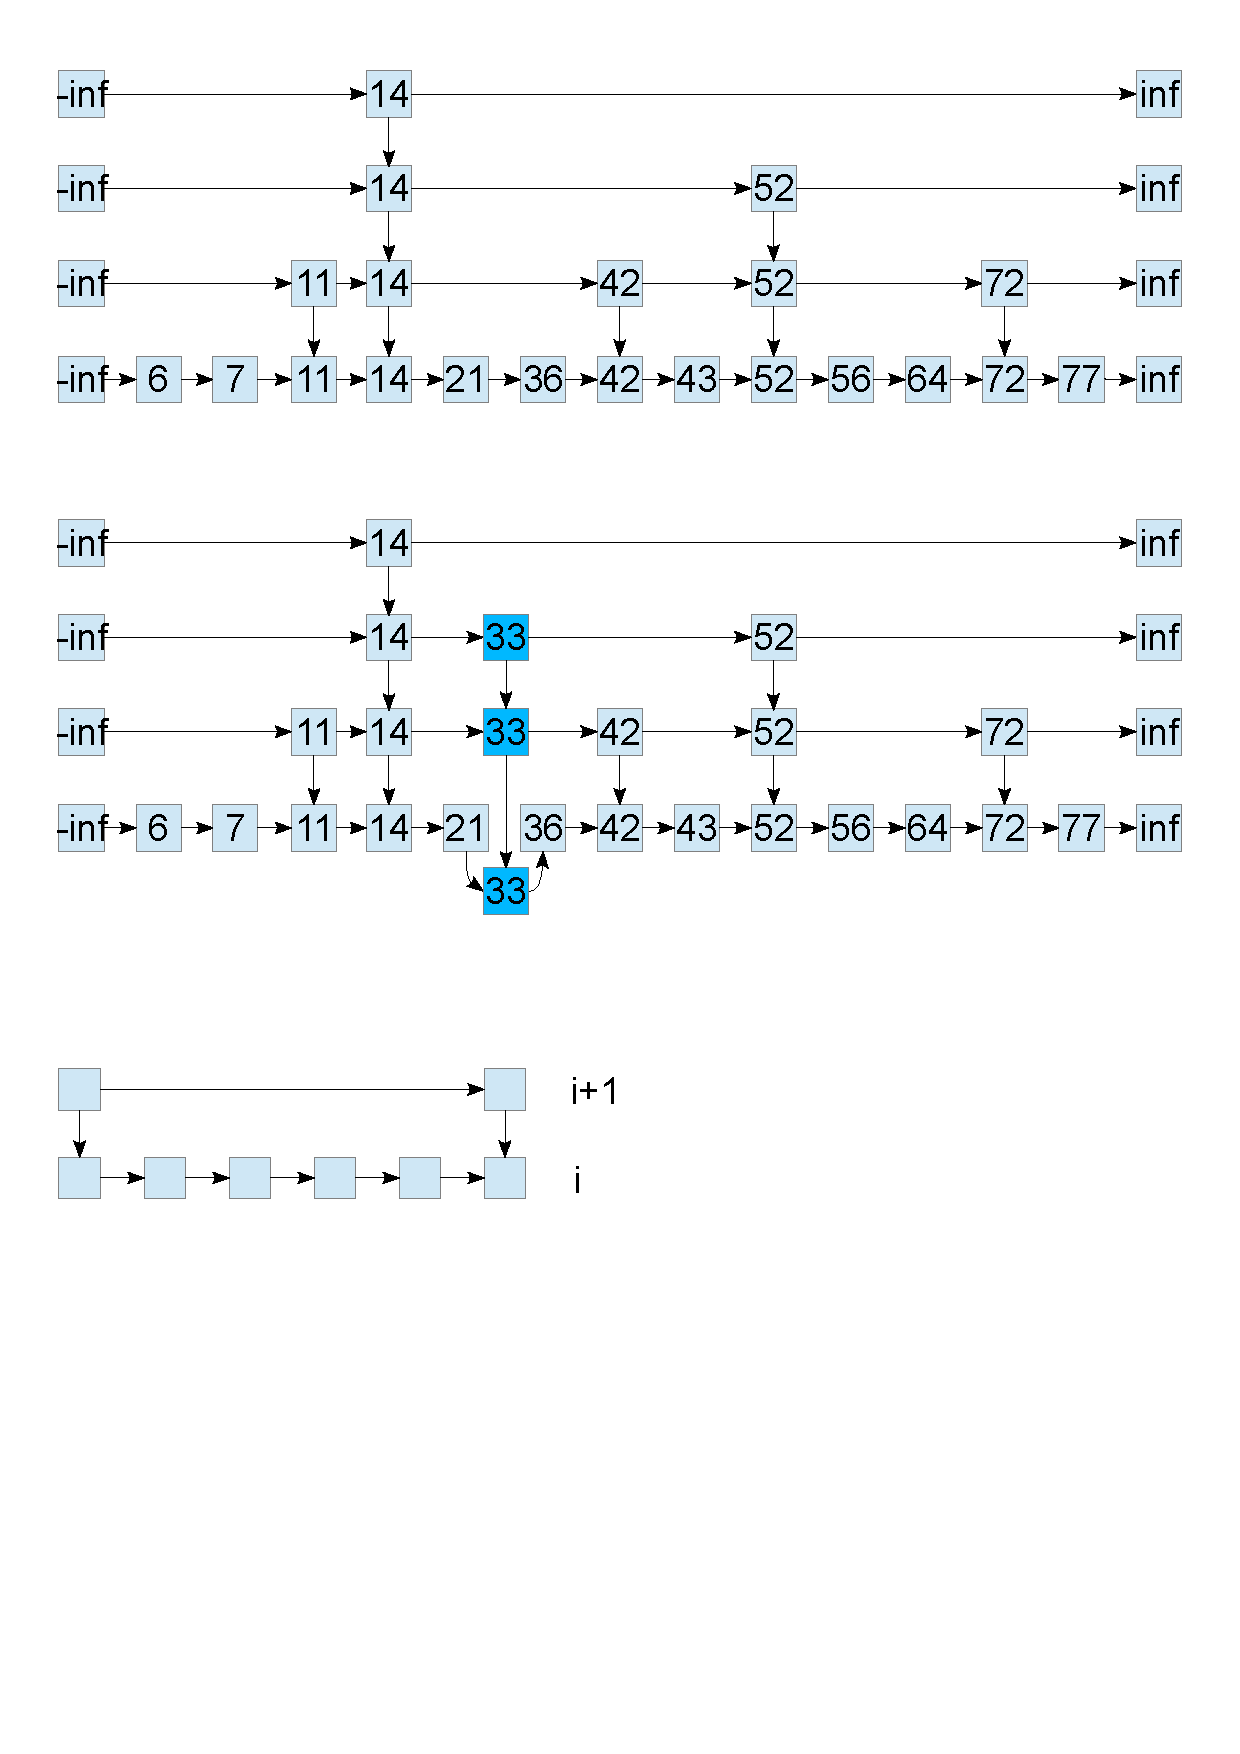
\includegraphics[trim= .9cm 9cm 8.9cm 18cm,clip,width=\columnwidth]{figures/skiplist.pdf}
\caption{In Skipliste einfügen}
\end{figure}
\begin{align*}\mathcal X = &\mbox{Zahl der Elemente auf Level i zwischen zwei}\\&\mbox{benachbarten Elementen auf Level i+1}\end{align*}
\[E(\mathcal X)=\sum_{j=1}^\infty j(1-p)^{j-1}p=p\frac{1}{(1-(1-p))^2}=\frac{1}{p}\]
Erwartete Suchzeit:
\[T_P(n)=\frac{1}{p}\log_\frac{1}{P}n=\mathcal O (\log n)\]
plot $\frac{x}{ln x}$ mit hervorheben des Sattelpunktes
\begin{align*}
f(x)&=x\log_xn\\
&=\frac{x\ln n}{\ln x}\\
f'(x)&=\ln n \frac{1\ln x -x\frac{1}{x}}{(\ln x)^2}=0\\
&\Rightarrow \ln x = 1\\
&\Rightarrow x=e \\
&\Rightarrow p=\frac{1}{e}
\end{align*}

\subsection{Dynamisches Programmieren}
es ist eine Technik um sich optimale Lösungen für Teilprobleme zu suchen.\\
\textbf{Beispiel:}\\
Sie sollen eine reihe von Matrizen multiplizieren. Die Dimensionen der Matrizen können durchaus unterschiedlich sein, was ist nun eine geschickte Reihenfolge um möglichst wenig Operationen zu benötigen?\\
geg: $n$-Matrizen $A_i$ für $i=1,\hdots,n$ , $A_i\in\mathbb R^{d_i\times d_{i+1}}$\\
ges: Optimale Auswerte-Reihenfolge für das Produkt $A_1 \dot A_2 \dot A_3 \dot \hdots \dot A_n$\\
Beispiel: $n=3$\\
\begin{align*}
(A_1 A_2) A_3 = 2 10 5 + 2 5 8 =180
A_1 (A_2 A_3) = 10 5 8 + 2 10 8= 560
\end{align*}

\[cost(A_i A_{i+1})=\theta(d_i d_{i+1} d_{i+2})\]
Bild 2\\
\[(A_1\hdots A_k)(A_{k+1}\hdots A_n)\]
\textbf{Idee:} Suche nach optimaler Teillösung und Konstruiere daraus die optimale Gesamtlösung.\\
\[cos(A_i a_{i+1} \hdots A_j)=c_{ij}\]
\[c_{ij}=\min_{i<k<j}c_{ik}+c_{k+1,j}+d_{i}d_{k+i}d_{j+1}\]




































































































\end{document}